\documentclass[parskip=half, bibliography=totoc]{scrartcl}
\usepackage{scrhack} % nach \documentclass
\usepackage[aux]{rerunfilecheck}
\usepackage{polyglossia}
\setmainlanguage{german}
\usepackage{fontspec}
\usepackage[unicode]{hyperref}
\usepackage{bookmark}
\usepackage[shortcuts]{extdash} %nach hyperref, bookmark
\usepackage[autostyle]{csquotes}
\setotherlanguages{english, french}
\usepackage{amsmath} % unverzichtbare Mathe-Befehle
\usepackage{amssymb} % viele Mathe-Symbole
\usepackage{mathtools} % Erweiterungen für amsmath
\usepackage{fontspec} % nach amssymb
\usepackage{booktabs}
\usepackage{longtable}
\usepackage{microtype}
\usepackage{xfrac}
\usepackage[
locale=DE,
separate-uncertainty=true, % Immer Fehler mit ±
per-mode=symbol-or-fraction,% m/s im Text , sonst \frac
% alternativ:
% per-mode=reciprocal, % m s^{-1}
% output-decimal-marker=.,  % . statt, für Dezimalzahlen
]{siunitx}
% Floats innerhalb einer Section halten
\usepackage[section, below]{placeins}
\usepackage{caption} % Captions schöner machen
\usepackage{subcaption}
\usepackage{graphicx}
\usepackage{grffile}
\usepackage{float}
\floatplacement{figure}{htbp}
\floatplacement{table}{htbp}
\usepackage[backend=biber]{biblatex}
\addbibresource{lit.bib}
\usepackage[
math-style=ISO, % \
bold-style=ISO, % |
sans-style=italic, % | ISO-Standard folgen
nabla=upright, % |
partial=upright, % /
]{unicode-math} % "Does exactly what it says on the tin."
\setmathfont{Latin Modern Math}
% \setmathfont{Tex Gyre Pagella Math} % alternativ
\usepackage[
version=4,
math-greek=default,
text-greek=default,
]{mhchem}

\begin{document}
\section{Theorie}
Das Trägheitsmoment ist das Massenäquivalent einer Translationsbewegung zu einer Rotationsbewegung. Die um eine Drehachse rotirende Punktmasse mit Masse $m$ und Abstand $r$ zur Rotationsachse besitzt ein Trägheitsmoment von $I = mr^2$.\\
Trägheitsmomente sind additiv.
Eine diskrete Anordnung von $n$ Punktmassen besitzt somit ein Gesamtträgheitsmoment aus der Summe der einzelnen Trägheitsmomente.
\begin{align*}
  I= \sum_{i = 0}^n r_i^2\cdot m_i
\end{align*}
Entsprechend gilt für eine kontinuierliche Masseverteilung
\begin{equation}
  \label{eqn:Trägheitsmoment}
  I = \int r^2 \mathup{dm}.
\end{equation}
In der Folgenden Aufzählung sind die Trägheitsmomente ausgewählter Geometrien aufgeführt.

\emph{Kugel}:
\begin{align*}
  I_K = \frac{2}{5}mR^2
\end{align*}
\emph{Zylinder}:
\begin{align*}
  I_{Zs} &= \frac{mR^2}{2} &
  I_{Zh} = m(\frac{R^2}{4} + \frac{h^2}{12})
\end{align*}
Wobei $I_{Zs}$ das Trägheitsmoment eines Zylinders bezüglich seiner Symmetrieachse und $I_{Zh}$ das Trägheitsmoment bezüglich der zur Symmetrieachse senkrechten Drehachse durch den Schwerpunkt ist.

Falls die Rotationsaches nicht durch den Schwerpunkt des rotierenden Körpers verläuft, sondern parrallel zu einer Schwerpunktsachse liegt, kann das Trägheitsmoment folgendermaßen berechnet werden
\begin{equation}
  \label{eqn:Steiner}
  I = I_S + m\cdot R^2.
\end{equation}
\begin{description}
  \item[$I_S$]Trägheitsmoment bezüglich der Schwerpunktsachse
  \item[$R$]Abstand der Drehachse zur Schwerpunktsachse
\end{description}
Die Gleichung \eqref{eqn:Steiner} ermöglicht es, dass nur das Trägheitsmoment, sowie der Abstand zu der parallelen Schwerpunktsachse benötigt wird, um das Trägheitsmoment bezüglich aller dazu parallelen Drehachsen zu bestimmen.
\subsection{Bestimmen der Trägheitsmomente}
Trägheitsmomente können über schwingungsfähige Systeme bestimmt werden. Die Schwingungsdauer und das Trägheitsmoment hängen folgendermaßen zusammen.
\begin{equation*}
  T = 2\pi \sqrt{\frac{I}{D}}
\end{equation*}
\begin{description}
  \item[$I$]Trägheitsmoment des Körpers
  \item[$D$]Winkelrichtgröße
\end{description}
Das Drehmoment ist das Kraftäquivalent bei einer Rotationsbewegung. Es ist definiert als $\vec{M} = \vec{F} \times \vec{r}.$ Mit einer anliegenden Kraft $\vec{F}$ und dem Abstand $\vec{r}$ von der Drehachse.
In dem Versuch wurden Torsionsschwingungen ausgenutzt, um die Trägheitsmomente zu berechnen. Der Betrag des Drehmoments kann über den Auslenkwinkel $\varphi$ und die Winkelrichtgröße der Feder $D$ berechnet werden. Dann ist $M = D\cdot sin(\varphi)$, bzw. kleinwinkelgenähert $M = D\cdot\varphi$.
\section{Durchführung}
Der Versuch wurde mit Hilfe einer Torsionsfeder realisiert. Der Aufbau des schwingenden Systems ist aus Abbildung \ref{fig:Aufbau} zu entnehmen.
\begin{figure}
  \centering
  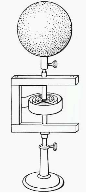
\includegraphics[height=4.00cm]{/home/sebastian/Bilder/V101_Aufbau.png}
  \caption{Experimenteller Aufbau.\cite{anleitung01}\protect}
  \label{fig:Aufbau}
\end{figure}
\FloatBarrier
\subsection{Winkelrichtgröße und Trägheitsmoment der Drillachse}
Zu Beginn des Versuches musste die Winkelrichtgröße der Feder und das Eigenträgheitsmoment der Drillachse ermittelt werden. Die Winkelrichtgröße wurde mit Hilfe einer Federwaage besstimmt, die in einem bestimmten Abstand sekrecht an einen Metallstange angebracht wurde. Die Metallstange ist durch die Drillachse verlegt und darf als masselos angenommen werden. Die Torsionsfeder wird ausgelenkt bis die Federwaage auf Null kallibriert wurde. Dann kann die Winkelskala eingestellt werden, sodass die Null mit der Auslenkung des Stabes übereinstimmt. Die Messung wird für drei verschiede Abstände und vier verschiedene Winkel durchgeführt. Die Winkelrichtgröße kann dann durch $D = \frac{F\cdot R}{\varphi}$ berechnet werden. $F$ ist die Federkraft, $R$ der Abstand und $\varphi$ der ausgelenkte Winkel.\\
Das Eigenträgheitsmoment der Drillachse wird dadurch bestimmt, dass zwei Gewichte an die Metallstange fixiert werden. Die Metallstange wird ausgelenkt, sodass das System zu schwingen beginnt. Die Periodendauer kann dann bestimmt werden. Die Messungen werden fünf mal für fünf Schwingungen durchgeführt. Insgesamt wird die Messung mit zehn verschiedenen Abstände realisiert.
\subsection{Trägheitsmoment zwei verschiedener Körper}
Zur Bestimmung des Trägheitsmomentes eines Körpers wird dieser auf der Drillachse befestigt und aus der Ruhelage ausgelenkt. Die Schwinungsdauer für fünf Schwingungen wird mithilfe einer Stoppuhr gemessen. Die Messung wird zehn mal wiederholt.
Es wurde das Trägheitsmoment der weißen Kugel und des grauen Zylinders bestimmt.
\subsection{Trägheitsmoment einer Holzpuppe}
In dem Experiment wird ausgenutzt, dass Trägheitsmomente additiv sind. Das Trägheitsmoment eines komplexen Körpers, wie zum Beispiel einer Holzpuppe kann dadurch approximiert werden, dass man den Körper in einfachere Geometrien zerlegt. Einfach Geometrien wie Zylinder oder Kugeln lassen sich schnell berechnen. Alle Trägheitsmomente bezüglich der selben Achse dürfen addiert werden.
Aus diesem Grund haben wir uns für folgende Stellungen der Holzpuppe entschieden.

\begin{figure}
  \centering
  \begin{subfigure}{0.48\textwidth}
    \centering
    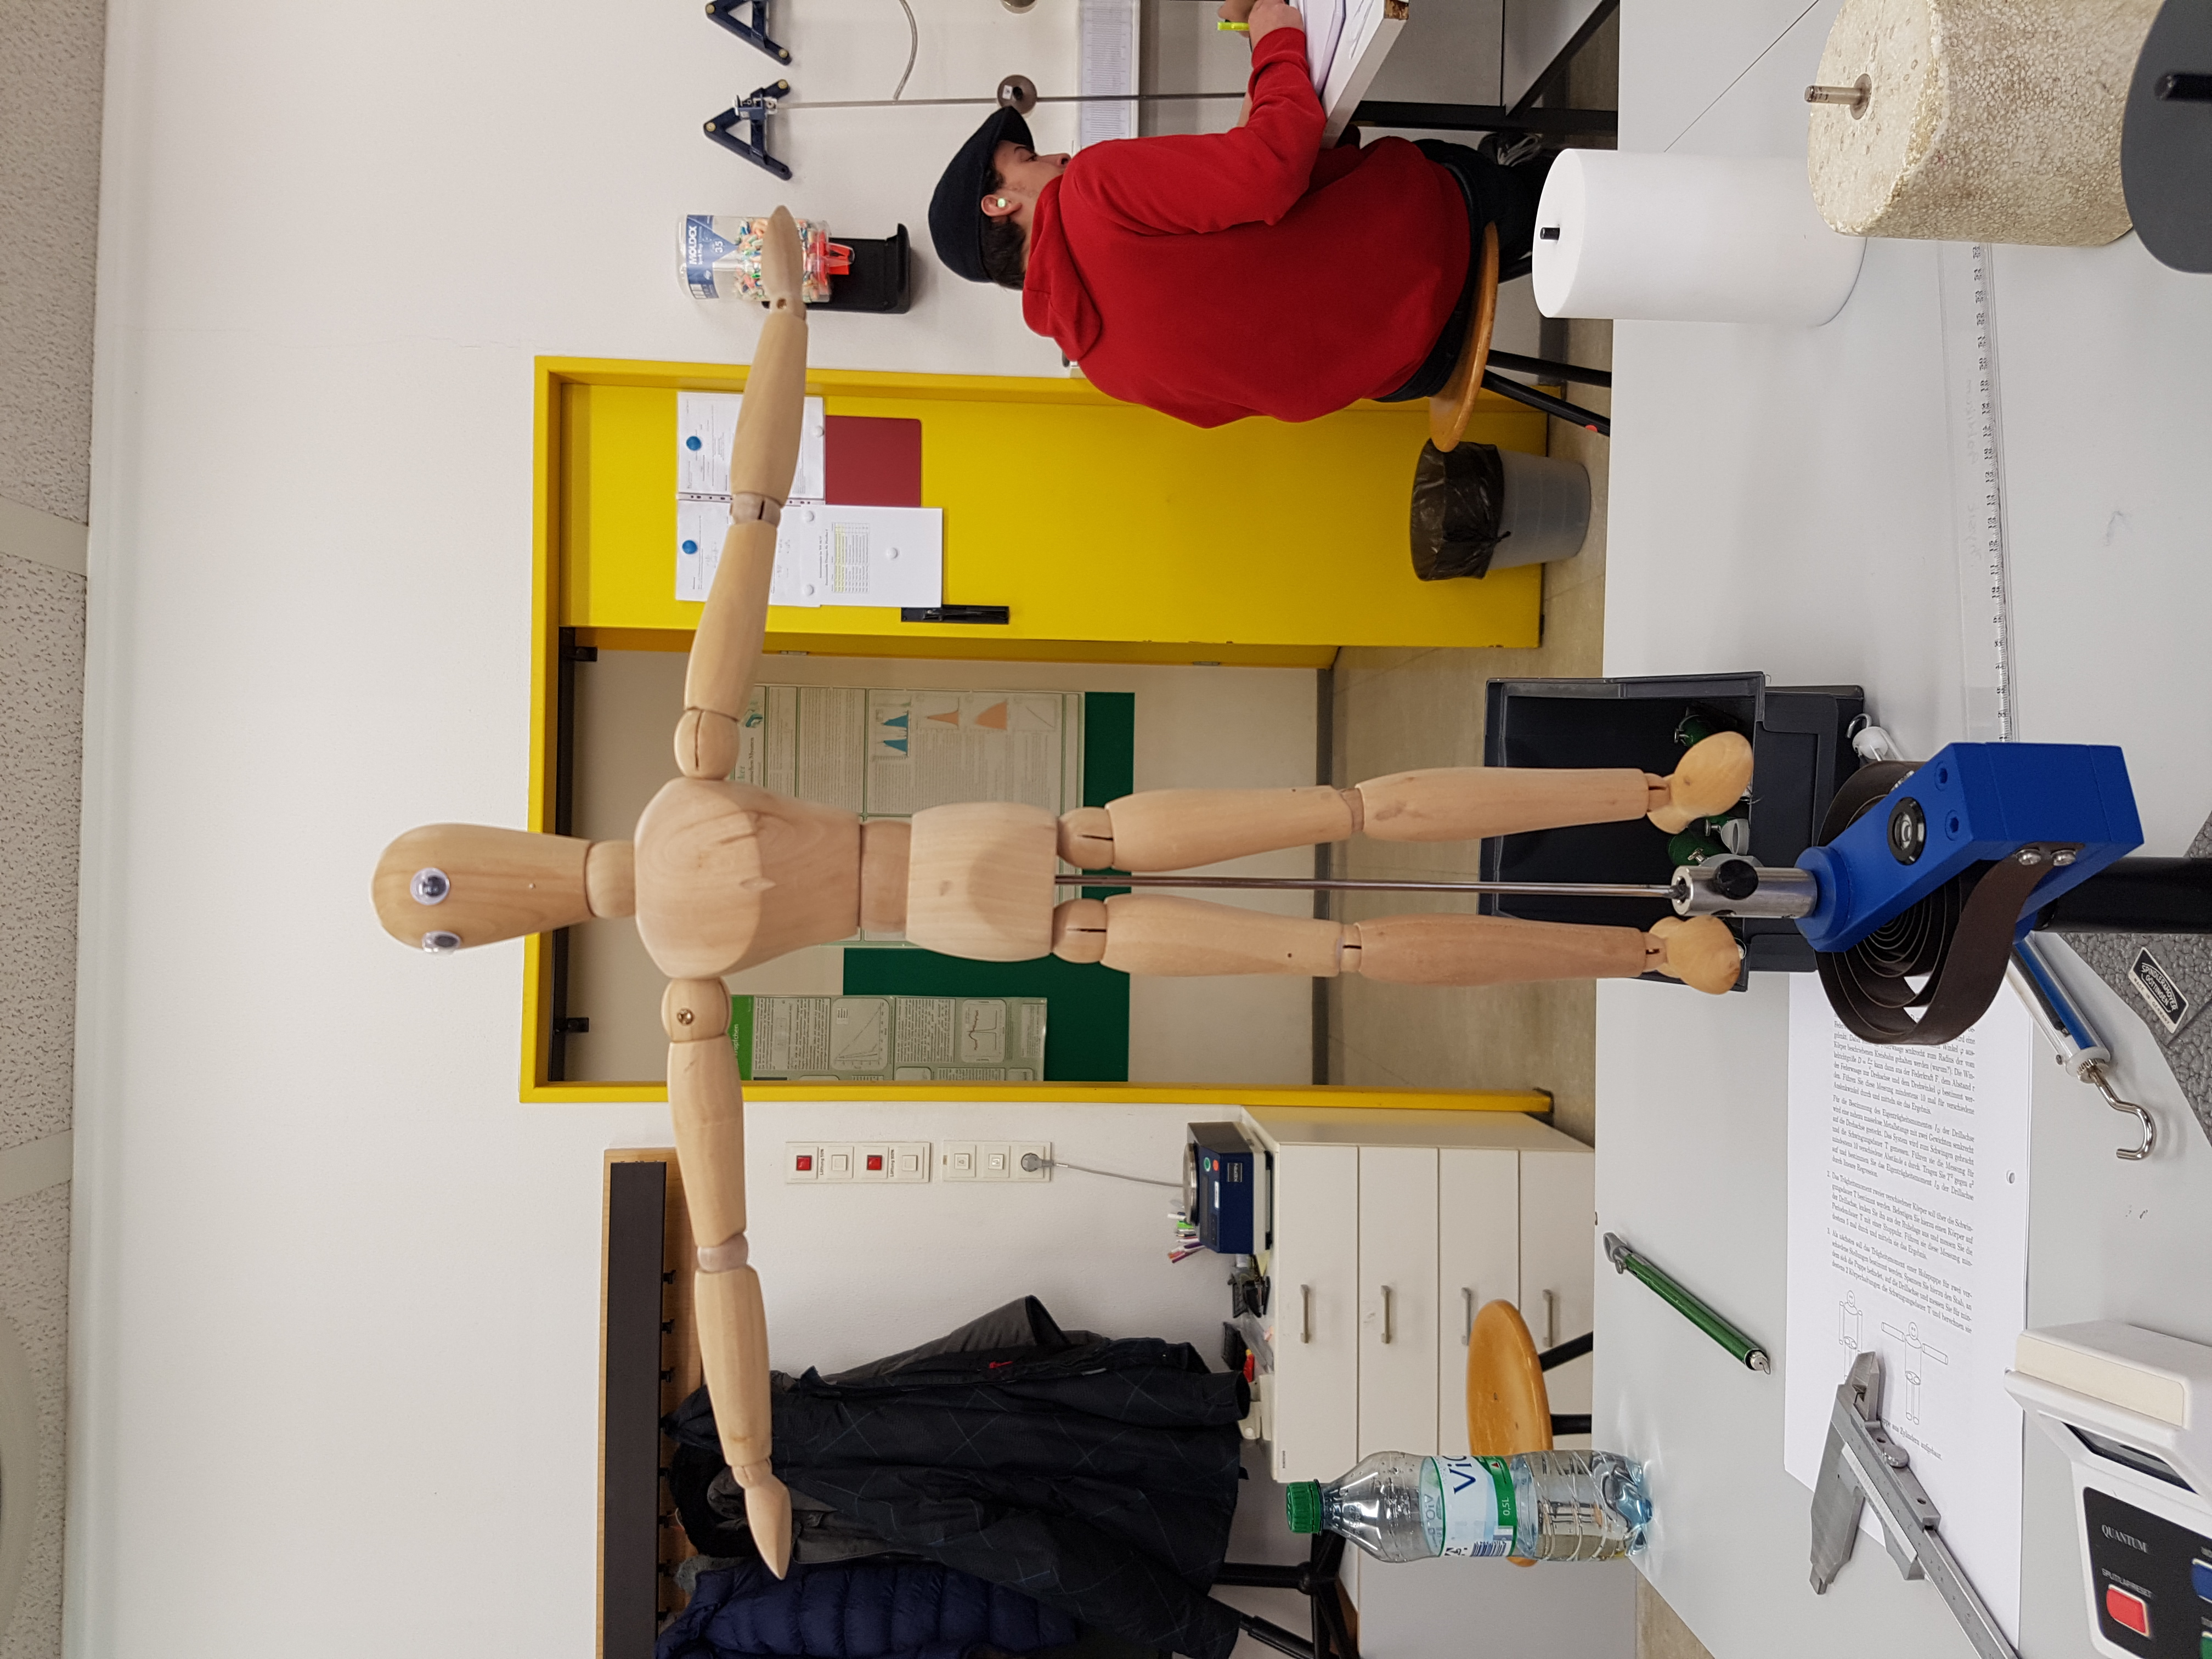
\includegraphics[height=3.00cm, angle=270]{/home/sebastian/Dokumente/Praktikum_TU_D_16-17/Protokolle/V101_Das_Trägheitsmoment/20161108_135922.jpg}
    \caption{Stellung a}
    \label{fig:stellunga}
  \end{subfigure}
  \begin{subfigure}{0.48\textwidth}
    \centering
    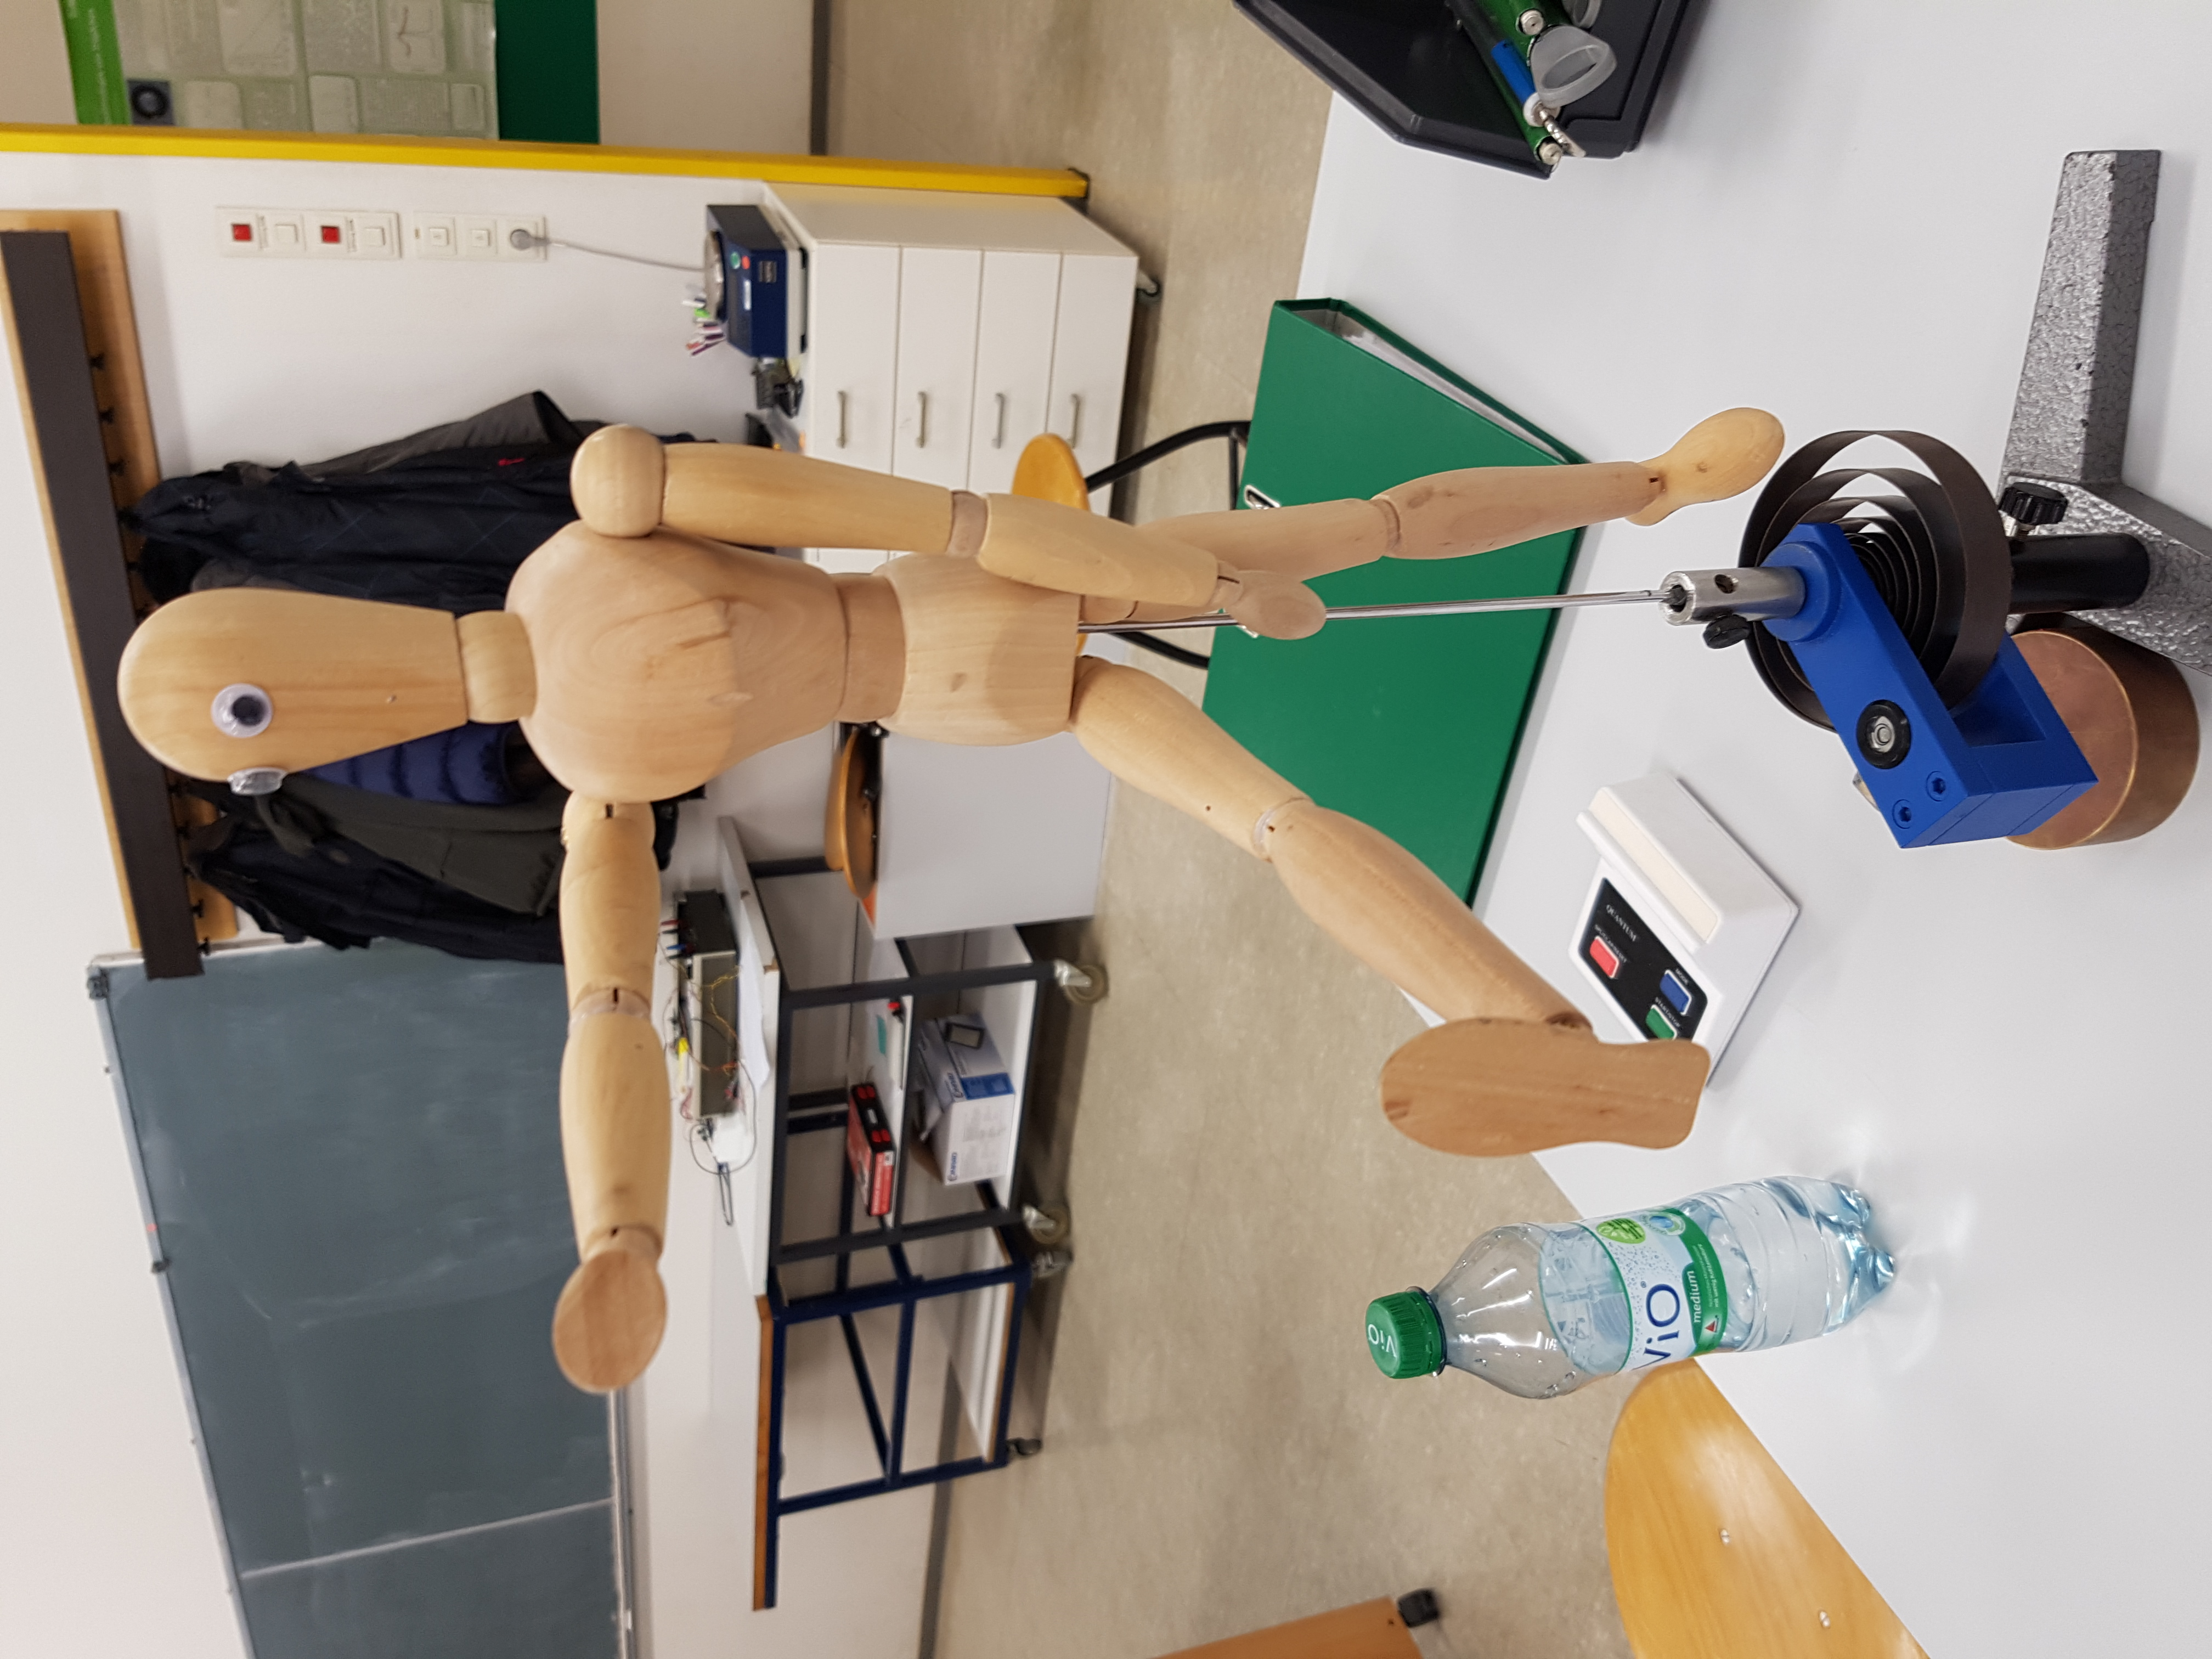
\includegraphics[height=3.00cm, angle=270]{/home/sebastian/Dokumente/Praktikum_TU_D_16-17/Protokolle/V101_Das_Trägheitsmoment/20161108_142542.jpg}
    \caption{Stellung b}
    \label{fig:stellunb}
  \end{subfigure}
  \label{fig:Holzpuppe}
\end{figure}

Somit haben alle einfachen Geometrien Trägheitsmomente bezüglich der selben Drehachse. Die Holzpuppe wird, in aufrechter Position auf die Drillachse eingespannt und es wird erneut die Schwingungsdauer von fünf Schwingungen genemssen. Die Messung wird zehn mal wiederholt.
\newpage
\printbibliography
\end{document}
